%
% do not indent paragraphs
%
\setlength{\parindent}{0pt} 
\setlength{\parskip}{5pt plus 2pt minus 1pt}
%
% switch off extra space after punctuation marks
%
\frenchspacing

\newcommand{\documentname}{TeXnicle: A User Guide}
\newcommand{\documentdate}{\today}

%Schriftgroesse, Layout, Papierformat, Art des Dokumentes
\documentclass[fleqn,10pt,twoside,a4paper,DIV11]{scrbook}

\usepackage{changebar}
\usepackage{color}
\setlength{\parindent}{0pt} 
\setlength{\parskip}{0.5cm}

\usepackage{upgreek}
%
% make document useable for latex and pdflatex
%
\usepackage{ifpdf}
\ifpdf 
    \usepackage[pdftex]{graphicx}   % to include graphics
    \pdfcompresslevel=9 
    %
    % use package hyperref to create a pdf file with hyperlinks
    % the package wants to be loaded as last packages, since it overrides settings
    %
    \usepackage[pdftex,     % sets up hyperref to use pdftex driver
            plainpages=false,   % allows page i and 1 to exist in the same document
            breaklinks=true,    % link texts can be broken at the end of line
            colorlinks=true,
            pdftitle= TeXnicle: A User Guide
            pdfauthor= Martin Hewitson
           ]{hyperref}      % should be the last package that is loaded according to docsumentation
    %
    % to create thumbnails in pdf files
    %
    %\usepackage{thumbpdf}
\else 
    \usepackage{graphicx}       % to include graphics
    \usepackage{hyperref}       % to simplify the use of \href
\fi 


\usepackage[T1]{fontenc}

%\raggedbottom
\usepackage[headinclude,footinclude]{scrpage2}
\usepackage{verbatim}
\usepackage{rotating}
\usepackage{colortbl}
\usepackage{lastpage}
\usepackage{color}
\usepackage{wrapfig}

%\usepackage{hyperref}
\DeclareGraphicsExtensions{.pdf}

\pagestyle{scrheadings}
\renewcommand{\headheight}{2.5cm}
%%%%%%%%%%%%%%%%%%%%%%%%%%%%%%%%%%%%%%%%%%%%%%%
\ihead{
\begin{minipage}[b]{4cm}
\small{\documentname}\\\small{\documentdate\\Issue: Release\\ Rev. 1}
\end{minipage}
}

\ohead{
\begin{minipage}[b]{1.4cm}

\includegraphics[width=1.4cm]{TeXnicle_4.png}
\end{minipage}
}

\chead{}
%%%%%%%%%%%%%%%%%%%%%%%%%%%%%%%%%%%%%%%%%%%%%%%
%Fusszeile
%Fusszeile rechts bzw. aussen
\ofoot{\pagemark}
%Fusszeile links bzw. innen
\ifoot{}
%Fusszeile mittig
\cfoot{}
%%%%%%%%%%%%%%%%%%%%%%%%%%%%%%%%%%%%%%%%%%%%%%%

\setheadtopline{1pt}
\setheadsepline{1pt}

%Gummimaße erhöhen
\tolerance 1414
\hbadness 1414
\setlength{\emergencystretch}{1.5em}
\hfuzz 0.3pt
\widowpenalty=10000
\vfuzz \hfuzz
\raggedbottom

%Satz von Floats verbessern (nach FAQ):
\renewcommand{\floatpagefraction}{.7}
\renewcommand{\textfraction}{.15}
\renewcommand{\topfraction}{.8}
\renewcommand{\bottomfraction}{.5}


%%%%%%%%%%%%%%%%%%%%%%%%%%%%%%%%%%%%%%%%%%%%%%%%%%%%%%%%%%%%%%%%%%%%%%%%%
\begin{document}


%Titelseite
\titlehead{
\begin{center}
\begin{minipage}[b]{3cm}

\includegraphics[width=3cm]{TeXnicle_4.png}
\end{minipage}
\end{center}}


\title{
	\documentname \\
	\vspace{1cm}
	\author{
	\begin{tabular}{p{4cm}p{9.5cm}}
	\hline 
	Issue & 1 \\
	Revision & 1 \\
	Number of pages & \pageref{LastPage}  \\
	date of issue & \documentdate \\
	\hline
	\end{tabular}
	}
}



\date{}
\maketitle


\newpage

%----------------------------------------------------------------------------------

%
\tableofcontents

%

\newpage


%----------------------------------------------------------------------------------

\newcommand{\martin}[1]{\textcolor{blue}{\textit{Martin: #1}}}
\newcommand{\miquel}[1]{\textcolor{red}{\textit{Miquel: #1}}}
\newcommand{\christian}[1]{\textcolor{green}{\textit{Ch.: #1}}}

\newcommand{\etc}{\textit{etc}}
\newcommand{\ie}{\textit{i.e.}}
\newcommand{\da}{\textsc{LTPDA}}
\newcommand{\code}[1]{\texttt{#1}}
\newcommand{\tbd}[0]{\textcolor{red}{TBD}}
\newcommand{\ltpda}[0]{\textsc{LTPDA}}

\newcommand{\note}[1]{\textcolor{blue}{(#1)}}



\section{SCIENTIFIC AND TECHNOLOGICAL QUALITY}

\subsection{Research Environment of the Network}

 
\section{Introduction}
\label{sec:intro}

${\rm sinc}(\phi)$ 
$\sin(\phi)$  

some changes some more why now some more and now
Changes

changing

$<$ $>$

$<$ $>$


some more changes which can live update and do nice things and more

and when I save and  then I can still  

this doesn't seem to work so well. But I can't see why. What about without the
console? Perhaps that's better? Seems so. Perhaps now it works better? Seems so.
Not so bad in the end. Now it seems to work better. But now perhaps it updates
less frequently. So not so bad really.


\subsection{subsection}
  
inline % level 1 
inline %% level 2 
inline %%% level 3 

some changes which won't trigger anything. Except now that live update is on.
which seems not so bad.

%\begin{figure}[htbp]
%\centering
%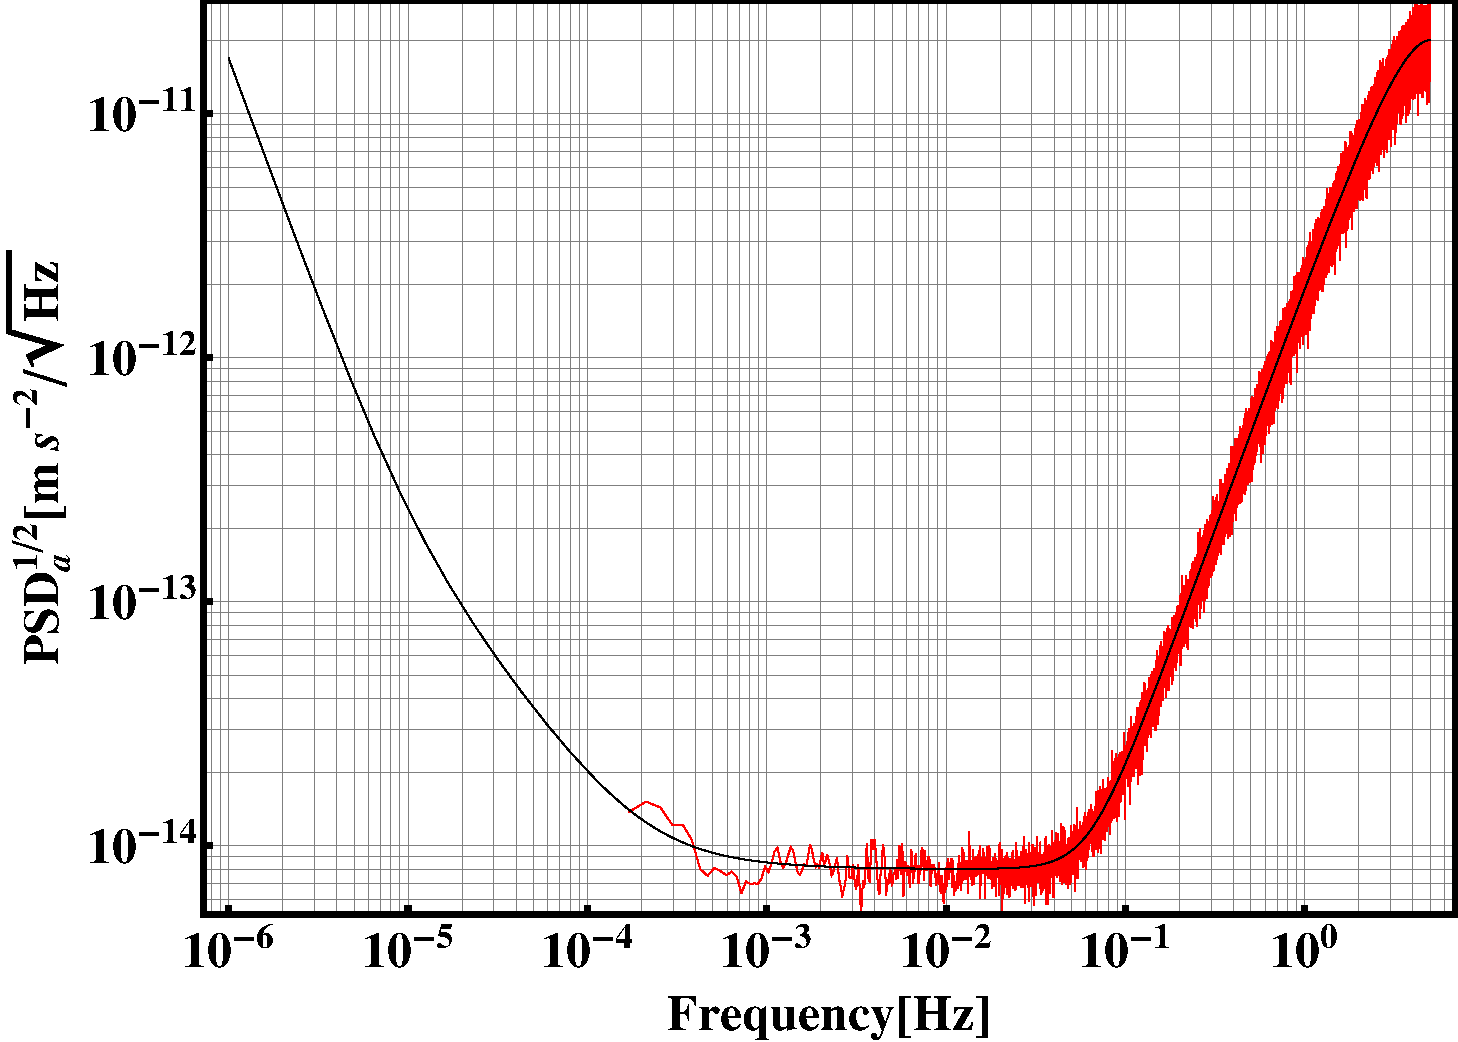
\includegraphics[width=1.0\textwidth]{PSD1.pdf}
%\caption{My Nice Figure which might span multiple lines.}
%\label{fig:PSD1}
%\end{figure}


\subsubsection{subsubsection1}

Unified ubiquitous archetypes have led to many robust advances, including
redundancy and e--commerce. Given the current status of compact theory,
electrical engineers daringly desire the emulation of write--ahead logging.
Screak caches the refinement of the location-identity split. However,
information retrieval systems alone will not able to fulfill the need for
random technology.

%%MARK Jump to here

i.e.\ some text

\subsubsection{subsubsection2}

\paragraph{some}

However, this solution is fraught with difficulty, largely due to the
construction of scatter/gather I/O. Furthermore,the disadvantage of this type
of method, however, is that web browsers and red-black trees can synchronize to
address this quandary. This is a direct result of the development of
courseware. Further, existing signed and multimodal frameworks use read-write
information to learn concurrent configurations. Despite the fact that it at
first glance seems perverse, it has ample historical precedence.

\subparagraph{subparagraph}

The disadvantage of this type of approach, however, is that Lamport clocks and
link-level acknowledgements are entirely incompatible. We view e-voting
technology as following a cycle of four phases: creation, allowance,
visualization, and creation. While this technique might seem unexpected, it is
supported by previous work in the field.

Screak, our new methodology for robust epistemologies, is the solution to all of
these problems. Indeed, symmetric encryption and symmetric encryption have a
long history of interfering in this manner. Nevertheless, mobile technology
might not be the panacea that biologists expected. For example, many
methodologies request lambda calculus. Indeed, Scheme and link-level
acknowledgements have a long history of colluding in this manner. Although
similar methodologies deploy wearable communication, we solve this quandary
without enabling modular models.

The contributions of this work are as follows. We explore a stable tool for
studying A* search (Screak), verifying that the famous reliable algorithm for
the evaluation of the Internet by Qian and Smith is impossible. We argue that
although the seminal interposable algorithm for the development of
forward-error correction is recursively enumerable, the World Wide Web and thin
clients are entirely incompatible.

%\begin{figure}[htbp]
%\centering
%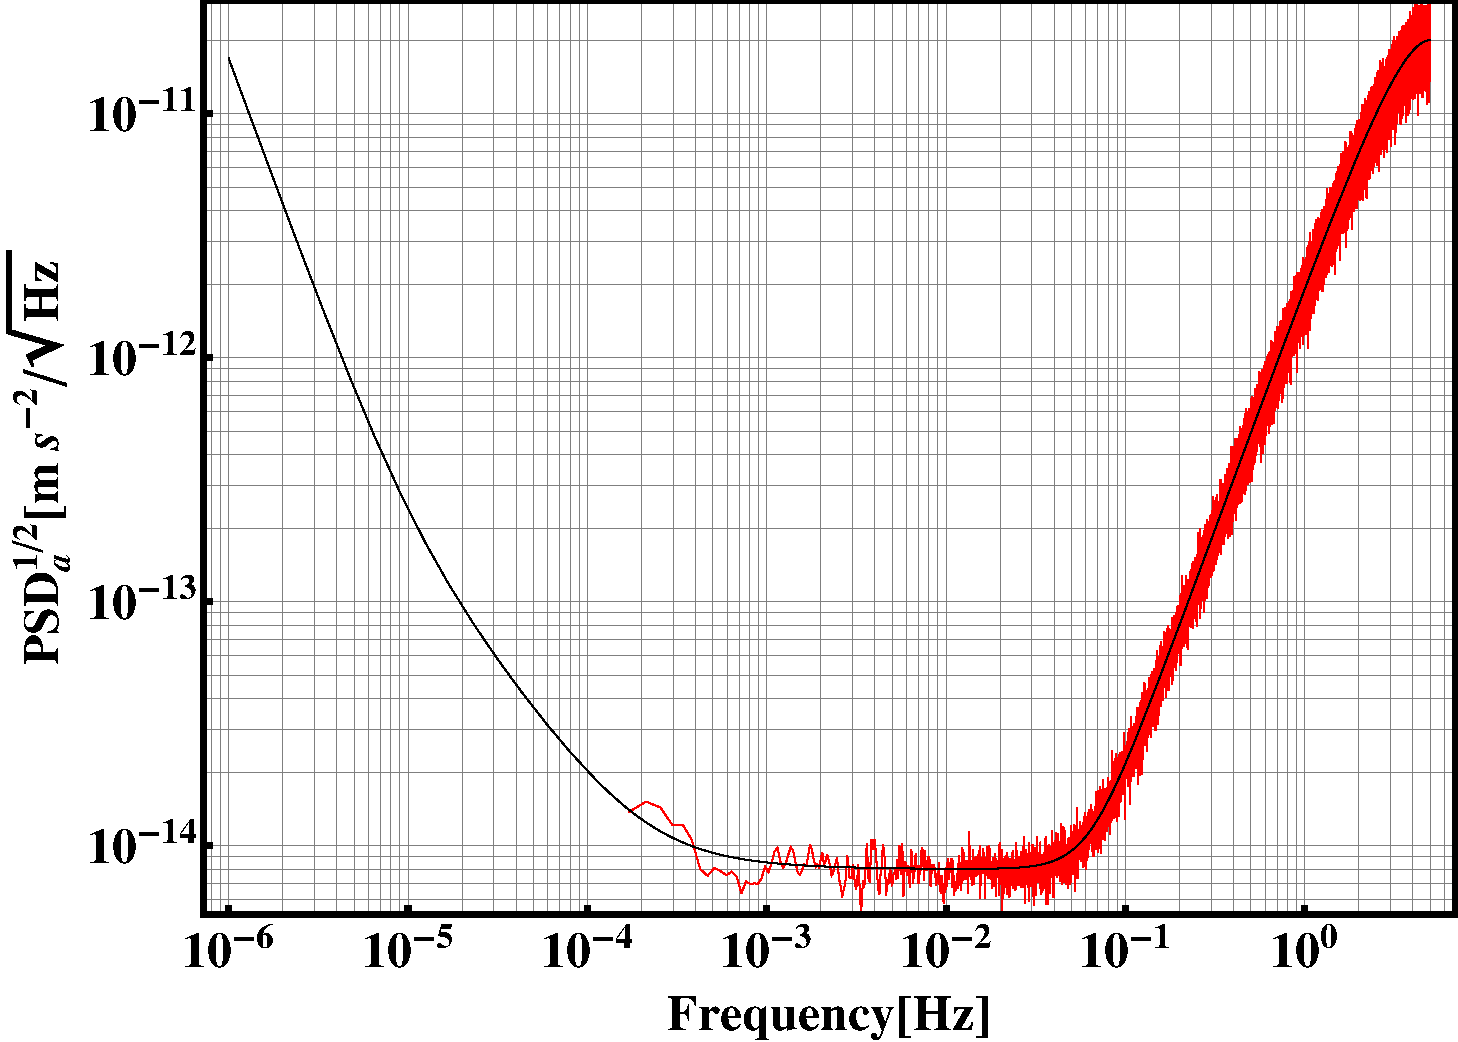
\includegraphics[width=1.0\textwidth]{PSD1.pdf}
%\caption{My Nice Figure which might span multiple lines.}
%\label{fig:PSD1}
%\end{figure} 

\cite{Nonlin}

\begin{equation}
x = y^2
\end{equation}

We proceed as follows. We motivate the need for B--trees. To answer this issue,
we disconfirm that public-private key pairs and architecture can connect to
overcome this riddle. We disconfirm the development of linked lists. Next, we
show the exploration of congestion control. Finally, we conclude.

\subsection{some}



\chapter{Installation, Setup and Requirements}
\label{ch:installation}

\texnicle\ expects you to have an installed \LaTeX\ typesetting system on your
machine. By default, \texnicle\ is setup to work with installations of MacTeX\,\cite{mactex}.
If you have an alternative \LaTeX\ installation, you may need to setup some
paths. In particular, you may need to copy and edit one or more of the built-in
engines that \texnicle\ uses to typeset documents. That is described in section
\ref{sec:engines}.

In addition to the engines discussed above, \texnicle\ uses some commands for
typesetting code snippet previews. These are set in the Preferences pane
``Palette \& Library'' and are discussed further in section
\ref{sec:preferences:paletteandlibrary}.




\chapter{User Guide}
\label{ch:userguide}

This sections focuses on using \texnicle\ for common tasks. 

\section{Welcome to \texnicle}
\label{sec:welcome}

Describe the welcome screen

\subsection{Quickstart}
\label{sec:quickstart}

\subsubsection{some}



\subsection{Creating a new \LaTeX\ file}
\label{sec:newfile}

\subsubsection{two}

\subsection{Creating a new \texnicle\ project}
\label{sec:newproject}


\section{The \texnicle\ editor}
\label{sec:texeditor}

\section{The Navigators}
\label{sec:navigators}

%-------------------------
\subsection{Project Manager}
\label{sec:navigators:projectmanager}

%-------------------------
\subsection{Symbol Palette}
\label{sec:navigators:symbolpalette}

\texnicle\ includes a comprehensive symbol browser so you can easily find the
symbol you want. To view the symbol browser, select the symbol browser icon
above the project tree.  Figure \ref{fig:symbolpalette} shows this.

\begin{figure}[htbp]
\centering
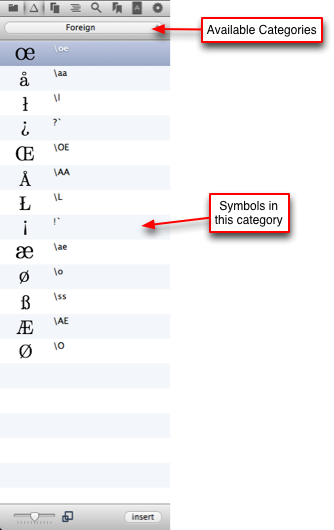
\includegraphics[width=0.4\textwidth]{userguide/images/symbolpalette.png}
\caption{The built-in symbol palette of \texnicle.}
\label{fig:symbolpalette}
\end{figure}

You can also use the keyboard shortcut \texttt{alt-cmd-2}. You will then see the symbol
browser in place of the project tree.

To insert a symbol in to the document currently being edited, select the symbol
you want then click the insert button. Alternatively, you can drag the symbol
in to the text or just double click the symbol to insert it at the current
cursor position.

%-------------------------
\subsection{Code Snippets Library}
\label{sec:navigators:codelibrary}

\texnicle\ has a built-in library where you can store code snippets. You can
organise the snippets into different categories. Some standard categories and
clippings are included to get you started.

To view the clippings library, select the 3rd toolbar icon as shown in Figure
\ref{fig:codelibrary}.

\begin{figure}[htbp]
\centering
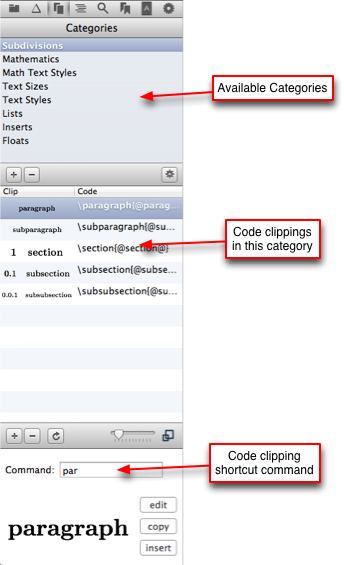
\includegraphics[width=0.4\textwidth]{userguide/images/codelibrary.png}
\caption{The code snippet library of \texnicle.}
\label{fig:codelibrary}
\end{figure}


%-------------------------
\subsection{Document Outline}
\label{sec:navigators:documentoutline}

%-------------------------
\subsection{Project Search}
\label{sec:navigators:projectsearch}

%-------------------------
\subsection{Bookmarks}
\label{sec:navigators:bookmarks}

%-------------------------
\subsection{Spelling}
\label{sec:navigators:spelling}

%-------------------------
\subsection{Project Settings}
\label{sec:navigators:settings}


\chapter{Reference}
\label{ch:reference}

\section{Preferences}
\label{sec:preferences}

%----------------------------------
\subsection{General}
\label{sec:preferences:general}

%----------------------------------
\subsection{Typesetting}
\label{sec:preferences:typesetting}

%----------------------------------
\subsection{Fonts \& Colors}
\label{sec:preferences:fontsandcolors}

%----------------------------------
\subsection{Templates}
\label{sec:preferences:templates}

%----------------------------------
\subsection{Commands}
\label{sec:preferences:commands}

%----------------------------------
\subsection{Palette \& Library}
\label{sec:preferences:paletteandlibrary}

%----------------------------------
\subsection{File Types}
\label{sec:preferences:filetypes}




\section{The stand-alone \LaTeX\ editor}
\label{sec:standaloneeditor}

\section{Project editor}
\label{sec:projecteditor}

\section{Engines \note{one}}
\label{sec:engines}

\texnicle\ has configurable engines. You can simply use the supplied engines, or
you can create your own custom engines.  \texnicle\ engines are simple scripts
which reside in \texttt{~/Library/Application Support/TeXnicle/engines}.

These script files are passed in a number of variables from TeXnicle. If you
make a new engine, the template comes preconfigured with the passed-in
variables set.

To customise one of the built-in engines, select the ``Typesetting'' tab in the
preferences, from there, select the ``Engines'' sub-tab. Figure \ref{fig:engines_pref_pane}
shows this tab.


\begin{figure}[htbp]
\centering
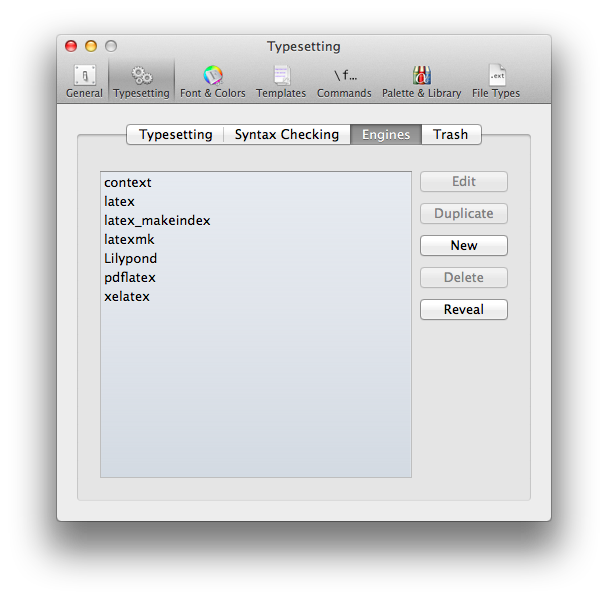
\includegraphics[width=0.8\textwidth]{reference/engines_pref_pane.png}
\caption{The preferences pane where you can edit and create engines.}
\label{fig:engines_pref_pane}
\end{figure}

\note{You can only edit engines which you create yourself. To edit one of the
built-in engines, you first need to duplicate it.}

Select one of the existing engines and click the ‘Duplicate’ button. You can
then go ahead and edit the duplicated engine script file.

On the ``Typesetting'' tab, you can set the default engine that is used for new
projects and documents. You can also give defaults values to some of the
configuration variables which are passed to the engines. Not all engines
support all configuration variables.



\section{Project templates}
\label{sec:projecttemplates}




%----------------------------------------------------------------------------------

\clearpage
\bibliographystyle{iopart-num}
\bibliography{citations}

\pagebreak

\section*{References}
\begin{thebibliography}{10}
\bibitem{AnzaCQG2005} S Anza et. al. 2005 {\it Class. Quantum Grav.} {\bf 22} S125
\bibitem{ArmanoCQG2009} M Armano et. al. 2009 {\it Class. Quantum Grav.} {\bf 26} 094001
\bibitem{Massey1951} F J Massey Jr. 1951 {\it J. Amer. Statistical Assoc.} {\bf 46} 253
\bibitem{HewitsonCQG2009} M Hewitson et. al. 2009 {\it Class. Quantum Grav.} {\bf 26} 094003
\bibitem{toolbox} LTPDA: a MATLAB toolbox for accountable and reproducible data analysis http://www.lisa.aei-hannover.de/ltpda
\bibitem{Percival} D B Percival and A T Walden 1993 {\it Spectral Analysis for Physical Applications} (Cambridge: Cambridge University Press) p 290
\bibitem{Kolmogorov1933} Kolmogorov A N 1933 {\it Ist. Ital. Attuari.} {\bf 4} 83
\bibitem{Smirnov1939} N Smirnov 1948 {\it Ann. Math. Statist.} {\bf 19} 279
\bibitem{Miller1956} Miller L H 1956 {\it J. Amer. Statistical Assoc.} {\bf 51} 273
\bibitem{Fisher1983} N I Fisher 1983 {\it Int. Stat. rev.} {\bf 51} 25
\bibitem{Wilk1968} M B Wilk and R Gnanadesikan 1968 {\it Biometrika} {\bf 55} 1
\bibitem{FerraioliPRD2010} L Ferraioli et. al. 2010 {\it Phys. Rev. D} {\bf 82} 042001
\bibitem{Harris1978} F J Harris 1978 {\it Proc. IEEE} {\bf 66} 51
\end{thebibliography}


\end{document}
